\documentclass{article}

\usepackage[utf8]{inputenc}
\usepackage[spanish]{babel}
\usepackage{graphicx}
\usepackage{hyperref}
\usepackage{cancel}
\usepackage{amsmath} % Este paquete define bmatrix
\usepackage{multirow, array} % para las tablas
\usepackage{float} % para usar [H]
\usepackage{array}
\usepackage{color}
\usepackage{colortbl}
\usepackage{multirow}

\definecolor{bg}{rgb}{0.95,0.95,0.95}

\begin{document}
	\title{Estad\'istica.  Seminario 2}
	\author{Daniel de la Cruz Prieto} 
	\maketitle
	
	\section*{Ejercicio 3 Clase Pr\'actica 5 }
	
		
		\begin{table}[ht]		
			\centering
			\begin{tabular}{|c|c|c|>{\columncolor[gray]{0.9}}c|}
				\hline 
				& Femenino & Masculino & $n_{i}*$ \\
				\hline
				Bueno(B) & 6 & 6 & 12 \\
				\hline
				Acecptable (A) & 7 & 6 & 13 \\
				\hline
				Malo (M) & 7 & 8 & 15 \\
				\hline
				\rowcolor[gray]{0.9} $n_{i}*$ & 20 & 20 & 40 \\
				\hline
			\end{tabular}
		\end{table}
		
		\begin{flushleft}
			\textbf{b-)} Decir si existe relaci\'on entre esas variables con un nivel de significaci\'on del~$5\%$.
		\end{flushleft}
		\begin{flushleft}
			Tomamos $ \alpha = 0.05$.
		\end{flushleft}
		
		\begin{flushleft}
			Estadigrafo :
		\end{flushleft}
		
		$$ x^2 = \sum_{i=1}^{y}\sum_{j=1}^{c}\frac{\left(n_{ij} - \frac{n_{i*}n_{*j}}{n}\right)^2}{\frac{n_{i*}n_{*j}}{n}}$$
		\begin{flushleft}
			$n_{ij} =$ frecuencia observada en la casilla i,j.
		\end{flushleft}
		\begin{flushleft}
			$e_{ij} = \frac{n_{i*}n_{*j}}{n} =$ frecuencia esperada en la casilla ij.
		\end{flushleft}
		
		\begin{equation*}
			\begin{array}{rcl}
			x^2 & = & \displaystyle \frac{\left(6 - \frac{12 * 20}{40}\right)^2}{\displaystyle \frac{12 * 20}{40}} + \displaystyle \frac{\left(6 - \frac{12 * 20}{40}\right)^2}{\displaystyle \frac{12 * 20}{40}}
			\\
			\\
			&  & + \displaystyle \frac{\left(6 - \displaystyle \frac{13 * 20}{40}\right)^2}{\displaystyle \frac{13 * 20}{40}} + \displaystyle \frac{\left(6 -  \displaystyle \frac{13 * 20}{40}\right)^2}{\displaystyle \frac{13 * 20}{40}}
			\\
			\\
			& & + \displaystyle \frac{ \displaystyle \left(6 - \frac{15 * 20}{40}\right)^2}{ \displaystyle \frac{15 \cdot 20}{40}} + \displaystyle \frac{ \displaystyle \left(6 - \frac{15 * 20}{40}\right)^2}{\displaystyle \frac{15 * 20}{40}}
			\\
			\\
			x^2 & = & 2\left[\frac{\left(-0.5\right)^2}{6.5}\right] + 2\left[\frac{\left(-1.5\right)^2}{7.5}\right]
			\\
			\\
			 & & + 2\left[\frac{0.25}{6.5}\right] + 2\left[\frac{2.25}{7.5}\right]
			\\
			\\
			x^2 & = & 2\left(0.038\right) + 2\left(0.3\right)
			\\
			\\
			x^2 & = & 0.076 + 0.6
			\\
			\\
			 x^2 & = & 0.676
			\end{array}
		\end{equation*}
		
		\begin{flushleft}
			\textbf{Regi\'on Cr\'itica:}
		\end{flushleft}
		
		\begin{equation*}    
		\begin{array}{rcl}
		X^2 & > & X_{1}^{2} - a \left(\left(r-1\right)\cdot \left(c-1\right)\right)\\\\
		 & > & X_{1}^{2} - 0.05 \left(\left(3-1\right)\cdot \left(2-1\right)\right)\\\\
		 & > & X^{2} - 0.95 \left(\left(2\right)\cdot \left(1\right)\right)\\\\
		0.676 = X^2 & > & X^{2} - 0.95 \left(2\right) = 5.99\\
		\end{array}
		\end{equation*}
		
		\begin{flushleft}
			Como la regi\'on cr\'itica no se cumple eso quiere decir que no rechaz\'o $H_{0}$ por lo que hay independencia entre las variables.
		\end{flushleft}
	
	
	
	\section*{Ejercicio 5 Clase Pr\'actica 5}
	
	\begin{flushleft}
		Para saber si existe relaci\'on entre las variables el coeficiente de correlaci\'on de Spearman pues los valores de la variables son ordinales
	\end{flushleft}
	
	\begin{table}[ht]
		\centering
		\begin{tabular}{|cccc|}
			\hline
			\rowcolor[gray]{0.9} X & Y & $d_{i}= X_i -Y_i$ & $d_{i}^{2}$ \\ 
			\hline
			1.00 & 1.00 & 0.00 & 0.00 \\ 
			2.00 & 2.00 & 0.00 & 0.00 \\ 
			3.00 & 3.00 & 0.00 & 0.00 \\ 
			4.00 & 4.00 & 0.00 & 0.00 \\ 
			5.00 & 5.00 & 0.00 & 0.00 \\ 
			\hline
	        &&& \cellcolor[gray]{0.9} 0.00  \\
			\hline
		\end{tabular}
	\end{table}
	
	\begin{flushleft}
		Con $n=5$ y los valores de la tabla calculamos entonces el coeficiente de r de Spearman.
	\end{flushleft}
	
	\begin{equation*}
		\begin{array}{rcl}
		r & = &\displaystyle 1- \frac{6 \cdot \sum d_{i}^{2}}{n\left(n-1\right)} \\
		r & = & 1 
		\end{array}
	\end{equation*}
	
	\begin{flushleft}
			Como $r=1$ podemos decir que existe correlacion entre las variables $X$ e $Y$
	\end{flushleft}

	\section*{Ejercicio 1 Clase Pr\'actica 6 }
	
	\begin{table}[ht]
		\centering		
		\begin{tabular}{|ccccc|}
			\hline
			\rowcolor[gray]{0.8} $X$ & $Y$ & $X\cdot Y$ & $X^2$ & $Y^2$ \\ 
			\hline
			-3.00 & 14.00 & -42.00 & 9.00 & 196.00 \\ 
			-1.00 & 4.00 & -4.00 & 1.00 & 16.00 \\ 
			1.00 & 2.00 & 2.00 & 1.00 & 4.00 \\ 
			3.00 & 8.00 & 24.00 & 9.00 & 64.00 \\ 
			5.00 & 22.00 & 110.00 & 25.00 & 484.00 \\ 
			\hline
			\rowcolor[gray]{0.9} 7.00 & 44.00 & 308.00 & 49.00 & 1936.00 \\ 
			\hline
		\end{tabular}
	\end{table}
	
	
	\begin{equation*}
		SS
	\end{equation*}

	\section*{Ejercicio 4 Clase Pr\'actica 5}
		\begin{flushleft}
			Para este ejercicio vamos a utilizar la correlaci\'on de $Pearson$ por ser esta una medida de la relaci\'on lineal entre dos variables aleatorias cuantitativas. Adem\'as que es independiente de la escala de la medida de las variables.
		\end{flushleft}

		\begin{table}[H]
		\centering
		\begin{tabular}{|c|c|c|c|c|}
			\hline
			x & y & $x\cdot y$ & $x^2$ & $y^2$ \\
			\hline
			10 & 12 & 120 & 10 & 144 \\
			\hline
			6 & 10 & 60 & 36 & 100 \\
			\hline
			5 & 15 & 75 & 25 & 225 \\
			\hline
			4 & 10 & 40 & 16 & 144 \\
			\hline
			3 & 13 & 39 & 9 & 144 \\
			\hline
			2 & 9 & 18 & 4 & 144 \\
			\hline
			5 & 15 & 15 & 25 & 144 \\
			\hline
			35 & 84 & 427 & 215 & 1044 \\
			\hline
		\end{tabular}
		\end{table}

		\begin{equation*}
		\begin{array}{rcl}
			r & = & \displaystyle \frac{n\sum_{i=1}^{n}\left(x_{i}y_{i}\right)-\left(\sum_{i=1}^{n}x_{i}\right)*\left(\sum_{i=1}^{n}y_{i}\right)}{\sqrt{\left(n\sum_{i=1}^{n}x_{i}^{2} - \left(\sum_{i=1}^{n}x_{i}\right)^2\right)\left(n\sum_{i=1}^{n}y_{i}^{2} - \left(\sum_{i=1}^{n}y_{i}\right)^2\right)}}\\\\
			r & = & \displaystyle \frac{7*\left(427\right)-\left(35\right)\left(84\right)}{\sqrt{\left(7*\left(215\right)-\left(35\right)^2\right)\left(7\left(1044\right)-\left(84\right)^2\right)}}\\\\
			r & = & \displaystyle \frac{2989 - 2940}{\sqrt{\left(1505 - 1225\right)\left(7308 - 7056\right)}}\\\\
			r & = & 0.18
		\end{array}
		\end{equation*}	
		
		\begin{flushleft}
			Como $r = 0.18$ entonces $-0.4 < r < 0.4$ y podemos decir que no existe correlaci\'on entre las variables, es decir no existe relaci\'on entre los resultados obtenidos en los recorridos de los algoritmos.
		\end{flushleft}
	
	\section*{Ejercicio 6 Clase Pr\'actica 6 }

		\subsection*{Contruya el diagrama de dispersi\'on .Parece ser lineal la relaci\'on?. Explique.}
			
			
		\begin{figure}[H]
			\centering
			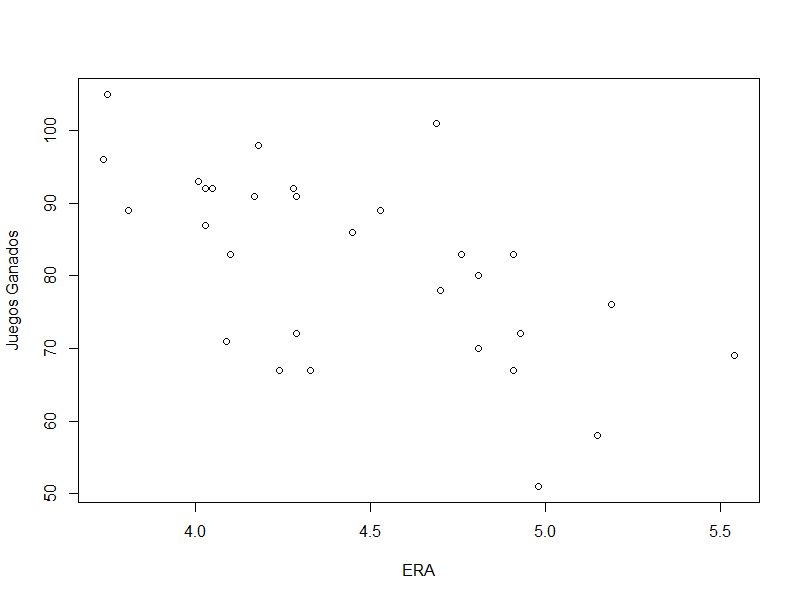
\includegraphics[width=0.9\textwidth]{img/DiagramadeDispersion.png}
			\caption{Diagrama de Dispersi\'on}
			\label{fig:ejemplo}
		\end{figure}
			



		\subsection*{El diagrama de dispersión sugiere que los equipos ganan más juegos cuando su ERA es más bajo? Explique.}
			
		\begin{flushleft}
		El diagrama de dispersi\'on sugiere que los equipo ganan m\'as juegos cuando su ERA es m\'as bajo pues a medida que aumenta el averaje los puntos tienden a estar m\'as cerca del eje de los(ERA)(en el gr\'afico es a las absisas).
		\end{flushleft}
	
	

		\subsection*{Encontrar la ecuaci\'on de la recta de mejor ajuste $x = ERA$ y $y = Juegos Ganados$.}
		
		\begin{flushleft}
			Ecuaci\'on de la recta :
		\end{flushleft}
			
		\begin{equation*}
			\begin{array}{rcl}
			\hat y & = & B_{0} + B_{1}x\\\\
			\hat y & = & 158.923 - 17.336 x
			\end{array}
		\end{equation*}
		
		    
		\subsection*{Trace la recta en el diagrama de dispersi\'on }
	
		\begin{figure}[H]
			\centering
			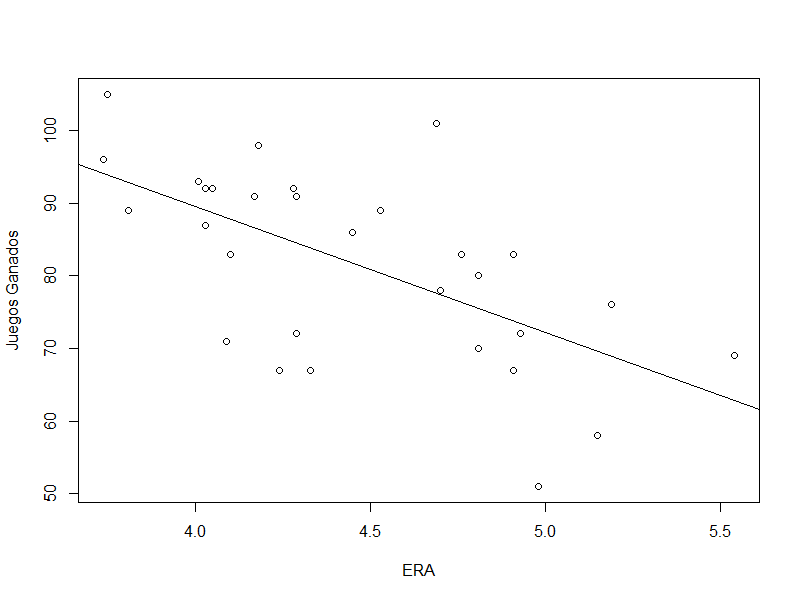
\includegraphics[width=0.9\textwidth]{img/DiagramadeDispersionConRectadeMinimoCuadrado.png}
			\caption{Diagrama de Dispersi\'on con la Recta de Mejor Aproximaci\'on}
		\end{figure}
		
			
		

		\subsection*{En promedio como se ve afectado el n\'umero de juegos ganados por un aumento unitario en el ERA.Explique como de termin\'o este n\'umero}

		\begin{flushleft}
			Como $\hat B_{1}$ representa el cambio pronosticado en la cantidad de juegos ganados por el aumento o disminuci\'on unitaria en el RAE. Entonces el n\'umero de juegos ganados $x$ se ve afentado en $-17.336 x$. Este n\'umero es la pendiente de la recta de mejor ajuste.
		\end{flushleft}

		\subsection*{Seg\'un sus concluciones. \textquestiondown Parece apoyar la idea de que los equipos con mejores porcentajes de ERA tendr\'an m\'as juegos ganados?. Justifique su respuesta. }

		\begin{flushleft}
			No, los equipos con mejores porcentajes de ERA tendr\'an menos juegos ganados seg\'un el diagrama de dispersi\'on. Pues la ecuaci\'on de la recta de menor ajuste tiene pendiente negativo.
		\end{flushleft}
		
		
		\section*{Ejercicio 1 Clase Pr\'actica 8}
		
		\begin{flushleft}
			Diagrama de Cajas
		\end{flushleft}
		
		\begin{figure}[H]
			\centering
			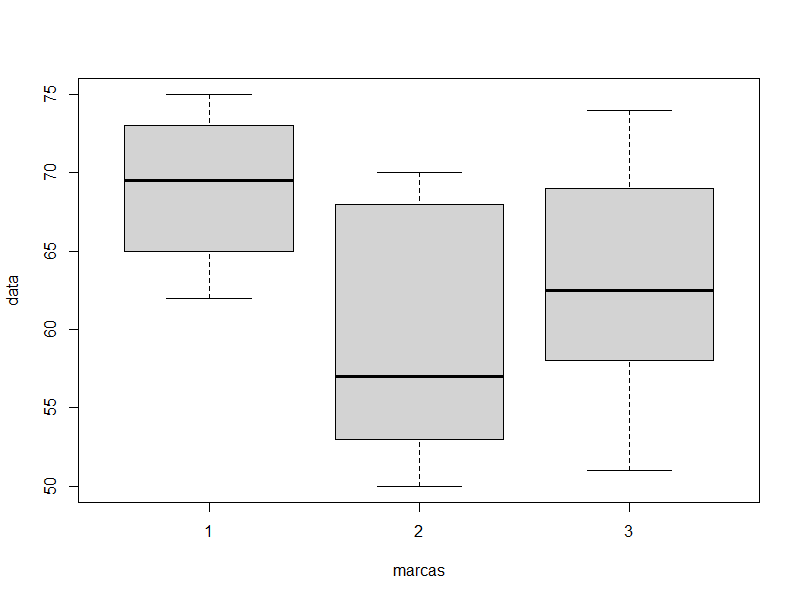
\includegraphics[width=0.9\textwidth]{img/ej1cp8-diagramadecajas.png}
			\caption{Diagrama de Cajas o Bigotes}
			\label{fig:ejemplo}
		\end{figure}
		
		
		\begin{flushleft}
			El diagrama de caja y bigote representa las tres marcas de spray donde se puede observar la media de
			efectividad de cada una, la que esta mas a la izquierda  la marca 1 que  tiene un promedio de efectividad de 69,
			la del centro  representa la marca n\'umero dos con un promedio de efectividad de aproximadamente 58 y por
			\'ultimo la que esta a la derecha  es la marca 3 con un promedio de efectividad de aproximadamente 63.
		\end{flushleft}
		
		\vspace*{1cm}
		
		\begin{flushleft}
			Gr\'afica de la muestra usando \textit{stripchart}
		\end{flushleft}
		
		\begin{figure}[H]
			\centering
			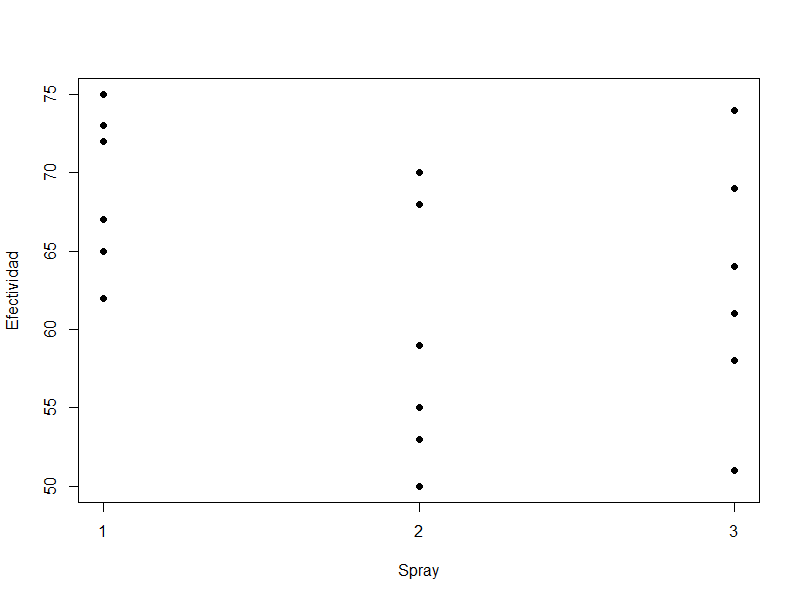
\includegraphics[width=0.9\textwidth]{img/ej1cp8-graficadelamuestra.png}
			\caption{Gr\'afica de la muestra }
			\label{fig:ejemplo}
		\end{figure}
		
		\begin{flushleft}
			Hip\'otesis
		\end{flushleft}
		
		$$
			H_0 = u_1 = u_2 = \dots = u_k = u
		$$
		
		$$
		H_1 = u_i=u_j \mbox{para alg\'un $i \neq j$}
		$$
		
		Donde $u_i$ es la efectividad de la marca de spray y $u$  es la media poblacional.
		
		
		\begin{flushleft}
			El modelo ser\'ia:
		\end{flushleft}
		
		$$
		Y_{ij} = u + a_i + e_{ij}
		$$
		
		Como el valor p = 0.0931 es mayor que la significaci\'on prefijada 
		$a=0.05$, no se rechaza $H_0$ y por tanto
		se asume que la media de la efectividad de los spray son iguales.
\end{document}